\section{Supplement to Section 2.6: the second data set}\label{supp:oz25}

\subsection{Data and digitisation}\label{supp:oz25-data}

\citet{ozsoy2025frequency} is open access (CC BY 4.0). Two groups of its tests were digitised: the stability lobe diagram of its Fig.~6 (DVF, $g=\SI{253}{\volt\second\per\metre}$, the structure of its Table~2, equal to Table~\ref{M-tab:case}), an embedded raster of $1428\times892$ pixels at 300 pixels per inch (1 pixel = \SI{2.09}{\rpm} = \SI{0.043}{\milli\metre}), and the saturation tests of its Figs.~10 and 12 (re-clamped structure, \SI{128.1}{\hertz}, \SI{1.48}{\percent}, \SI{1.13e7}{\newton\per\metre}), the first drawn as vector graphics, the second an embedded raster of $1521\times842$ pixels at 300 pixels per inch. Each figure was digitised twice, independently, from the pixels of a 600-dpi rendering: the axes were calibrated on at least two labelled ticks or gridlines (residuals below \SI{0.21}{pixel} for Fig.~6), every marker or label was located in the pixels and checked on an overlay drawn on the figure. Fig.~6 holds 49 markers: 28 controlled stable cuts, 9 controlled chatter, 2 controlled marginal, 1 controlled loss of contact, 2 uncontrolled stable, 3 uncontrolled chatter and 4 onsets of saturation in the article's time-domain simulation; every unoccluded marker lies within \SI{1}{\rpm} and \SI{0.03}{\milli\metre} of a round value, and the lettered cuts A--H reproduce the values given in the article's text. Figs.~10 and 12 hold 56 annotated tests: the measured amplitude of the command in newtons (36) or `Sat' (20), with the outcome `chatter' (5) or `marginal' (3) where given; the labels are left-aligned at the test speed and centred on the test depth, every centre within \SI{0.061}{\milli\metre} of a round depth, and each value of Fig.~10 equals that at the same place in Fig.~12 where the latter shows it (52 of 56). The two digitisations agree on all 49 markers and on all 56 values and outcomes, on the stability curves of Fig.~10 to \SI{0.08}{\milli\metre}, and on those of Fig.~6 to \SI{0.09}{\milli\metre} (controlled) and \SI{0.23}{\milli\metre} (uncontrolled, on the narrow lobes below \SI{700}{\rpm}; \SI{0.06}{\milli\metre} above).
% src: verification/ozsoy2025/digitise_notes.md, points_fig6.json, points_fig10.json

\subsection{Linear limits}\label{supp:oz25-lin}

Outside the steep flanks of the lobes, where the limit of the model changes by more than \SI{0.2}{\milli\metre} per rpm (1, 5, 1 and 1 of the 109, 109, 23 and 23 digitised points), the uncontrolled and controlled ($g=\SI{253}{\volt\second\per\metre}$) limits of the model with the structure of Table~\ref{M-tab:case} deviate from the digitised curves of Fig.~6 by 0.04 and \SI{0.14}{\milli\metre} RMS (median relative deviation 0.3 and \SI{3}{\percent}), and with the re-clamped structure from those of Fig.~10 by 0.06 and \SI{0.07}{\milli\metre}; with all points, by 0.04, 0.15, 0.08 and \SI{0.07}{\milli\metre}. A least-squares fit of the gain to the controlled curve of Fig.~10 gives \SI{251}{\volt\second\per\metre}. Fig.~\ref{fig:oz25-sld} places the 49 markers of Fig.~6 on the model's chart: the linear limit predicts 26 of the 39 controlled cuts reported stable, marginal or chattering and 4 of the 5 uncontrolled ones; the article's own controlled curve, interpolated at the test speeds, predicts the same 26. The cut with loss of contact (D in the article, \SI{2800}{\rpm}, \SI{5.5}{\milli\metre}), reported stable but with broadband vibration that the article attributes to loss of contact between the actuator assembly and the workpiece, lies above both limits and is not classified. The two controlled cuts that lost stability between the limits, G (marginal) and H (chatter) at \SI{2100}{\rpm} and 5 and \SI{6}{\milli\metre}, lie above the onset of saturation of the article's simulation at that speed (\SI{4.5}{\milli\metre}), and the article attributes H to the command exceeding the linear range of the actuator; the forced demand of the model there is 14.1 and \SI{14.7}{\newton}. The simulated face and step entries with the \SI{9}{\volt} clip give the same classification as the linear limit at all 39 controlled cuts: the forced demand of these cuts stays below \SI{27}{\newton} (at most \SI{25.8}{\newton}, at \SI{2000}{\rpm} and \SI{5}{\milli\metre}).
% src: verification/ozsoy2025/fit_gain.json (points kept by fit_gain.compare, model slope <= 0.2 mm/rpm: 108/109, 104/109, 22/23, 22/23; RMS with all points, from the rows: 0.041, 0.154, 0.076, 0.073 mm; fig6 uncontrolled rms 0.040 mm, median_rel 0.003; controlled_g253 rms 0.137 mm, median_rel 0.030; fig10_uncontrolled rms 0.062 mm; fig10_gain_fit g_best 251, rms_at_253 0.074 mm); compare2025.json (fig6.by_type: controlled_stable 28, linear_unstable 11; controlled_chatter 9, linear_unstable 8; controlled_marginal 2, linear_unstable 1; uncontrolled_chatter 3, linear_unstable_uncontrolled 2; uncontrolled_stable 2, 0; sim_face_chatter equal to linear_unstable in every type); paper/figures/figure_numbers.json (fig_oz25_sld n_mismatch 14 including the uncontrolled chatter at 2100 rpm / 2.5 mm)

\begin{figure}[!htbp]
  \centering
  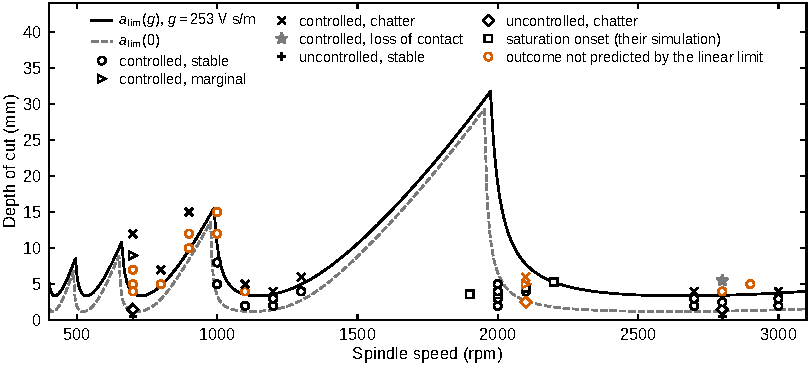
\includegraphics[width=\textwidth]{figures/fig_oz25_sld.pdf}
  \caption{The cuts of Fig.~6 of \citet{ozsoy2025frequency} (structure of Table~\ref{M-tab:case}, DVF, $g=\SI{253}{\volt\second\per\metre}$) on the linear limits of the model; orange markers: outcome not predicted by the linear limit (controlled cuts: the controlled limit; uncontrolled cuts: the uncontrolled limit); the cut with loss of contact (grey) is not classified. The squares are the onsets of saturation of the article's time-domain simulation, not tests.}
  \label{fig:oz25-sld}
\end{figure}

\subsection{Forced command, saturation and outcome of the saturation tests}\label{supp:oz25-sat}

For every test of Figs.~10 and 12 (Table~\ref{tab:oz25}), the settled forced demand $F_p=K_ag\max\lvert\dot x_p\rvert$ was computed from 40 tooth-passing harmonics of the helical force applied to the controlled receptance, which is the forced command of Section~\ref{M-sec:model-orbit} in force units ($F_p>\SI{27}{\newton}$: the forced orbit reaches the \SI{9}{\volt} clip); the alternative readings of a measured `amplitude', the amplitude of the tooth-passing harmonic and $\sqrt2$ times the RMS value, differ from $F_p$ by less than \SI{2}{\percent} median ratio. Each test was simulated with the face and the step entry, the \SI{9}{\volt} clip, the full surface memory and loss of contact, and classified by D1 over the 300 revolutions after full engagement; whether the command reached the clip at any time of the run was recorded. Between the two linear limits the critical kick was computed at the phases 0, 4, 8 and 12 of 16 with the protocol of Section~\ref{M-sec:bistab-prot}. In Table~\ref{tab:oz25}, Meas.\ is the measured amplitude of the command, or Sat where it saturated; Out.\ the measured outcome (C chatter, M marginal, otherwise stable); Pos.\ the depth relative to the limits of the model (B below $\alim(0)$, W between $\alim(0)$ and $\alim(g)$, A above $\alim(g)$); $F_p$ the predicted settled forced demand; Face and Step the simulated outcome with each entry (S settles, C chatters; $^*$: the command reaches the clip during the run); and $\Delta v^*$ the smallest critical kick over the four phases, for the tests between the limits ($\infty$: no chatter up to \SI{3}{\metre\per\second}).

\begin{table}[!htbp]
  \centering
  \caption{Saturation tests of \citet{ozsoy2025frequency} (Figs.~10 and 12) against the model (columns defined in Section~\ref{supp:oz25-sat}).}
  \label{tab:oz25}
  \scriptsize
  \setlength{\tabcolsep}{4pt}
  \renewcommand{\arraystretch}{0.84}
  \begin{tabular}{@{}rrrcrrccr@{}}
    \toprule
    $n$ & $a$ & Meas. & Out. & Pos. & $F_p$ & Face & Step & $\Delta v^*$\\
    (rpm) & (mm) & (N) & & & (N) & & & (mm/s)\\
    \midrule
1700 & 3 & 9 &  & B & 8.4 & S & S & \\
1700 & 5 & 12 &  & B & 11.4 & S & S & \\
1700 & 10 & 10 &  & B & 7.4 & S & S & \\
1700 & 15 & 5 &  & B & 7.0 & S & S & \\
1700 & 20 & 13 &  & A & 11.5 & C & C & \\
1750 & 2 & 9 &  & B & 7.4 & S & S & \\
1750 & 3 & 12 &  & B & 10.4 & S & S & \\
1750 & 5 & 14 &  & B & 14.4 & S & S & \\
1750 & 10 & 9 &  & B & 9.2 & S & S & \\
1750 & 15 & 4 &  & B & 8.8 & S & S & \\
1750 & 20 & 16 &  & A & 14.5 & C & C & \\
1800 & 0.5 & 3 &  & B & 2.5 & S & S & \\
1800 & 1.5 & 8 &  & B & 7.3 & S & S & \\
1800 & 3 & 13 &  & B & 13.6 & S & S & \\
1800 & 5 & 19 &  & B & 18.8 & S & S & \\
1800 & 10 & 15 &  & B & 12.0 & S & S & \\
1800 & 15 & 6 &  & B & 11.4 & S & S & \\
1800 & 20 & Sat &  & W & 19.0 & S & S & $\infty$\\
1800 & 22 & 19 &  & A & 14.1 & C & C & \\
1850 & 2 & 15 &  & B & 13.3 & S & S & \\
1850 & 3 & 20 &  & B & 18.8 & S & S & \\
1850 & 5 & Sat &  & B & 25.8 & S* & S & \\
1850 & 10 & Sat &  & B & 16.6 & S & S & \\
1850 & 15 & 6 &  & B & 15.8 & S & S & \\
1850 & 20 & Sat &  & B & 26.1 & S* & S & \\
1900 & 0.5 & 5 &  & B & 4.5 & S & S & \\
1900 & 1.5 & 12 &  & B & 13.2 & S & S & \\
1900 & 3 & Sat &  & B & 24.5 & S* & S & \\
1900 & 5 & Sat &  & B & 33.8 & S* & S* & \\
1900 & 10 & Sat &  & B & 21.5 & S* & S & \\
1900 & 15 & 8 &  & B & 20.6 & S* & S & \\
1900 & 20 & Sat &  & B & 34.1 & S* & S* & \\
1950 & 2 & 19 &  & B & 16.5 & S & S & \\
1950 & 3 & Sat &  & B & 23.5 & S* & S & \\
1950 & 5 & Sat &  & B & 32.7 & S* & S* & \\
1950 & 10 & Sat &  & B & 20.6 & S* & S & \\
1950 & 15 & 16 &  & W & 19.7 & S* & S* & $\infty$\\
1950 & 20 & Sat & M & W & 33.0 & S* & S* & 397\\
2000 & 2 & 14 &  & B & 12.6 & S & S & \\
2000 & 3 & 19 &  & B & 18.0 & S & S & \\
2000 & 5 & Sat &  & W & 25.0 & S* & S* & $\infty$\\
2000 & 10 & Sat & M & W & 15.7 & S & S* & 139\\
2050 & 2 & 12 &  & B & 9.7 & S & S & \\
2050 & 3 & 16 &  & B & 13.7 & S & S & \\
2050 & 5 & Sat & C & W & 18.8 & S* & S* & $\infty$\\
2050 & 10 & Sat & C & A & 12.1 & C* & C* & \\
2100 & 2 & 10 &  & B & 7.8 & S & S & \\
2100 & 3 & 13 &  & W & 10.9 & S & S & $\infty$\\
2100 & 5 & Sat & C & W & 14.8 & S & S* & $\infty$\\
2100 & 10 & Sat & C & A & 9.6 & C* & C* & \\
2150 & 2 & 7 &  & W & 6.4 & S & S & $\infty$\\
2150 & 3 & 11 &  & W & 9.0 & S & S & $\infty$\\
2150 & 5 & Sat & M & W & 12.2 & S & S & $\infty$\\
2200 & 2 & 7 &  & W & 5.5 & S & S & $\infty$\\
2200 & 3 & 18 &  & W & 7.7 & S & S & $\infty$\\
2200 & 5 & Sat & C & A & 10.3 & C & S & \\
    \bottomrule
  \end{tabular}
\end{table}
% src: verification/ozsoy2025/sim2025.py/.json (closed_form.demand_N, face/step chatter and run_clipped), compare2025.json (fig10.rows position; amplitude_h1 and amplitude_rms2 median ratios 0.888 and 0.889 against 0.903 for the peak), kicks2025.json

Of the 36 numerical values, the predicted $F_p$ is 0.90 times the measured one (median; interquartile range 0.83--1.02; correlation 0.66): 0.92 (range 0.82--1.10) at the 16 tests of up to \SI{5}{\milli\metre} at 1700--\SI{2000}{\rpm}, with absolute errors of at most \SI{2.5}{\newton}, 0.81 (range 0.43--0.92) at the 8 tests of up to \SI{5}{\milli\metre} from \SI{2050}{\rpm}, 0.80 at \SI{10}{\milli\metre}, 2.05 (range 1.23--2.64) at \SI{15}{\milli\metre} and 0.89 at 20--\SI{22}{\milli\metre}. The settled forced orbit is predicted to saturate at 4 of the 20 saturated tests (1900 and \SI{1950}{\rpm}, 5 and \SI{20}{\milli\metre}), the command reaches the clip during the simulated face entry at 12 of them and at 2 unsaturated ones (1900 and \SI{1950}{\rpm}, \SI{15}{\milli\metre}), and later in the run at 2 more saturated ones (2050 and \SI{2100}{\rpm}, \SI{10}{\milli\metre}), through simulated chatter above the controlled limit. The simulated face entry chatters exactly at the six tests above the controlled limit, of which three were measured stable; it settles at all 13 tests between the limits, of which five lost stability.
% src: verification/ozsoy2025/compare2025.json (fig10.amplitude_peak; demand_over_measured; abs_error_depth_le5_rpm_le2000_N max 2.46; saturation_settled_closed_form both 4; saturation_any_time_face_entry both 14, pred_only 2; outcome_face both 3, pred_only 3, meas_only 5)

\paragraph{Helix angle} From 1700 to \SI{1950}{\rpm} the measured command has a local minimum over the depth near \SI{15}{\milli\metre}, between the two regions of saturation, while the tooth-passing force of the \SI{45}{\degree} helix is most nearly constant at the axial pitch, $\pi D/(N_t\tan45^\circ)$, which is \SI{12.6}{\milli\metre}. Recomputed with helix angles of 36--\SI{46}{\degree}, everything else unchanged, the mean absolute logarithmic ratio of predicted to measured command at the 36 tests falls from 0.24 at \SI{45}{\degree} to 0.16 at \SI{42}{\degree} (axial pitch \SI{14.0}{\milli\metre}). This only locates the discrepancy, in the distribution of the force, or of the mode, over the depth; the model keeps the \SI{45}{\degree} of the article.
% src: verification/ozsoy2025/helix2025.py/.json (mean_abs_log 0.240 at 45, 0.159 at 42 (best), 0.164 at 43; pitch_mm 12.57 and 13.96)

\paragraph{Onset of saturation in the article's simulation} The four squares of Fig.~6, the article's time-domain onsets of saturation at 1900, 2000, 2100 and \SI{2200}{\rpm}, lie at 3.6, 3.6, 4.5 and \SI{5.3}{\milli\metre}; the forced demand of the model reaches \SI{27}{\newton} at 4.1 and \SI{5.9}{\milli\metre} at the first two speeds and not below the controlled limit at the others (\SI{13.5}{\newton} at \SI{2100}{\rpm} and \SI{4.5}{\milli\metre}; at \SI{2200}{\rpm} the square, at \SI{5.29}{\milli\metre}, lies on the model's controlled limit of \SI{5.28}{\milli\metre}). The details of that simulation are not given.
% src: verification/ozsoy2025/onset2025.py/.json (model_onset_mm 4.15, 5.90, None, None: first depth of a 0.05 mm grid with demand above 27 N; closed form 26.94 N at 4.10 mm, 27.02 N at 4.12 mm, 27.00 N at 5.85 mm; square at 2200 rpm digitised at 5.292 mm (points_fig6.json depth_measured_mm); demand_at_article_onset_N 24.8, 21.3, 13.5, 9.6; a_lim_g_mm 2200 rpm 5.280)
